\documentclass[letterpaper,10pt,conference]{ieeeconf}
\IEEEoverridecommandlockouts
\overrideIEEEmargins
\usepackage[T1]{fontenc}
\usepackage{amsmath,amssymb}
\usepackage{balance}
\usepackage{tikz}
\usetikzlibrary{arrows.meta}
\usepackage[hidelinks]{hyperref}
\hypersetup{pdftitle={Local and Global Identifiability Can Differ in Linear Networks},
 pdfauthor={Anders Hansson},
 pdfsubject={Draft for IEEE Control Systems Letters},
 pdfkeywords={identification, linear networks, local identifiability, global identifiability}}
\newtheorem{theorem}{Theorem}
\newtheorem{proposition}{Proposition}
\newtheorem{lemma}{Lemma}
\newcommand{\diag}{\operatorname{diag}}
% L-CSS requires a citation to the AI system in each section using AI text.
% The acknowledgment describes the scope of this assistance.
\newcommand{\aicite}{\texorpdfstring{\protect\cite{codex}}{}}

\title{\LARGE\bf
Local and Global Identifiability Can Differ in Linear Networks}
\author{Anders Hansson, \textit{Senior Member, IEEE}%
\thanks{Anders Hansson is with the Division of Automatic Control,
Link\"oping University. Email:
\href{mailto:anders.g.hansson@liu.se}{\texttt{anders.g.hansson@liu.se}}.}}

\begin{document}
\maketitle
\thispagestyle{empty}
\pagestyle{empty}

\begin{abstract}
For a linear network, the network matrix collects complex coefficients that relate
its node signals. Local identifiability means that the observed response
to external inputs uniquely determines all sufficiently close admissible
coefficient vectors; global identifiability requires uniqueness among all
admissible vectors. For scalar coefficients, generic means that exceptions have zero volume in
parameter space. We show that generic local identifiability does not imply
generic global identifiability when only selected nodes receive inputs and
are measured. A six-node network with nine independent unknown coefficients
has exactly two compatible vectors generically. Adding six nodes, each
supplied with an input and measured, preserves the ambiguity and allows
both compatible network matrices to have spectral radius, the largest
eigenvalue magnitude, below any prescribed positive bound. The resulting
structure has twelve nodes, forty-two independent unknown coefficients,
and zero diagonal. Ambiguity persists on a nonempty open set of the full
parameter space, with both candidates satisfying the same spectral-radius
bound. An explicit rational pair has exact matrix-power bounds.
The constant coefficients also define proper transfer functions:
rational functions whose numerator degree does not exceed their
denominator degree.
Replacing scalar coefficients by rational transfer functions preserves
the two-solution construction.
\end{abstract}

\begin{keywords}
Identification, network analysis and control, linear systems.
\end{keywords}

\section{Introduction \aicite}\label{sec:intro}

A linear network consists of node signals related by linear equations
along prescribed directed edges. An external input excites a node when it
enters that node's equation; a measurement records a selected node signal.
Network identification seeks to recover the unknown edge coefficients from
the response of the measured signals to the external inputs. When only
some nodes are excited or measured, distinct choices of internal
coefficients can produce the same observed response.

Local identifiability means that the coefficients are unique among
sufficiently close admissible choices. Global identifiability requires
uniqueness among all admissible choices. For scalar coefficients,
a property is called generic if it holds except on a set of parameter
values of zero volume.
The distinction matters when a test based on derivatives establishes
local uniqueness: such a test need not exclude a second, isolated
explanation of the same input-output relation.

Legat and Hendrickx developed a generic local identifiability test for
partial excitation and measurement and asked whether local and global
identifiability can differ in this setting \cite{LH20}. The two notions
coincide when all nodes are excited or all nodes are measured
\cite{LH24}. A further equivalence result holds for a specified class
of two-part networks with known internal coefficients \cite{LH23}.
The general question remains open in the
discussion of \cite[Sec.~II-C]{LH24} and
\cite[Sec.~12.2]{L25}. The latter reports an unsuccessful search for a
counterexample with up to five unknown edges, subject to specified
structural restrictions.

This letter gives a negative answer for networks with independently
unknown complex scalar coefficients and fixed selections of excited and measured
nodes. First, a six-node construction has exactly two compatible
coefficient vectors generically. Second, adding excited and measured
nodes preserves the
ambiguity while controlling the spectral radius, the largest magnitude
of a matrix eigenvalue. Both alternatives satisfy the restriction on this
quantity imposed in \cite{LH24}. The augmented structure has twelve
nodes and forty-two independently unknown coefficients. For every positive
bound on the spectral radius, ambiguity occurs on a nonempty open subset
of the full parameter space of forty-two complex coefficients.

Section~\ref{sec:setting} states the admissible classes and the precise
identifiability definitions. Sections~\ref{sec:base} and
\ref{sec:augmentation} develop the two constructions.
Section~\ref{sec:main} proves the spectral-radius result and gives an
explicit rational pair. Section~\ref{sec:conclusion} extends the result
to rational transfer functions under an algebraic definition of generic
identifiability.

\section{Network Description and Identifiability \aicite}
\label{sec:setting}

A transfer function describes a linear relation between signals in the
frequency domain. We follow the scalar formulation of
\cite[Secs.~I and III]{LH20} and \cite[Sec.~III-B]{LH24}: each edge
coefficient represents a transfer-function value at a fixed frequency and
can therefore be complex.

Let \(n\) be the number of nodes, numbered \(1,\ldots,n\), and let \(E\)
be a prescribed set of ordered pairs \((i,j)\), where
\(i,j\in\{1,\ldots,n\}\) and \(i\ne j\). An edge
\((i,j)\) carries the signal from node \(j\) to node \(i\).
Write \(m=|E|\), fix an ordering of these edges, and collect their
coefficients in a vector \(\theta\in\mathbb C^m\). The network matrix
\(G(\theta)\in\mathbb C^{n\times n}\) places these coefficients in the
positions in \(E\) and has zeros elsewhere. Each edge has its own
independent parameter. In particular, \(G(\theta)\) has zero diagonal.

Let \(n_B\) and \(n_C\) be the numbers of excited and measured nodes.
The fixed matrix \(B\in\{0,1\}^{n\times n_B}\) has distinct columns of
the identity matrix, and \(C\in\{0,1\}^{n_C\times n}\) has distinct rows
of the identity matrix. Thus \(B\) inserts inputs at the excited nodes
and \(C\) selects the measured signals. At the chosen frequency, let
\(w\in\mathbb C^n\), \(r\in\mathbb C^{n_B}\), and
\(y\in\mathbb C^{n_C}\) be the complex amplitudes of the node signals,
inputs, and measurements, respectively. The network equations are
\begin{equation}\label{eq:network}
 w=G(\theta)w+Br,\qquad y=Cw.
\end{equation}
For a positive integer \(d\), let \(I_d\) denote the \(d\times d\)
identity matrix. We call \eqref{eq:network} well posed if
\(I_n-G(\theta)\) is invertible. In that case the transfer matrix
from the external inputs \(r\) to the measurements \(y\), evaluated
at the chosen frequency, is
\begin{equation}\label{eq:observation}
 \Phi(\theta)=C(I_n-G(\theta))^{-1}B.
\end{equation}
Identification concerns recovery of \(\theta\) from \(\Phi(\theta)\).

Define the set of well-posed parameters by
\[
 \Omega=\{\theta\in\mathbb C^m:\det(I_n-G(\theta))\ne0\}.
\]
For a matrix, let \(\rho\) denote its spectral radius. For
\(0<\varepsilon\le1\), define the more restricted set
\begin{equation}\label{eq:domain}
 \Omega_\varepsilon
   =\{\theta\in\mathbb C^m:\rho(G(\theta))<\varepsilon\}.
\end{equation}
The strict inequality implies \(\Omega_\varepsilon\subseteq\Omega\).
Openness and volume are understood by identifying \(\mathbb C^m\)
with \(\mathbb R^{2m}\) through real and imaginary parts.
Both parameter sets are open in this topology.

Let \(\mathcal D\) be either \(\Omega\) or \(\Omega_\varepsilon\).
The network is \emph{locally identifiable at \(\theta\in\mathcal D\)}
if some neighborhood \(N\) of \(\theta\) satisfies the following
implication for every alternative vector \(\widetilde\theta\):
\[
 \widetilde\theta\in N\cap\mathcal D,\quad
 \Phi(\widetilde\theta)=\Phi(\theta)
 \quad\Longrightarrow\quad \widetilde\theta=\theta.
\]
It is \emph{globally identifiable at \(\theta\) in \(\mathcal D\)}
if the same implication holds for every
\(\widetilde\theta\in\mathcal D\). Thus any competing network must satisfy
the same admissibility restriction.

The structure is generically locally or globally identifiable in
\(\mathcal D\) if the corresponding property holds outside a subset of
\(\mathcal D\) of Lebesgue measure zero, that is, zero volume.
We use the complex Jacobian, the matrix of derivatives of the entries
of \(\Phi\) with respect to the complex coordinates of \(\theta\).
All ranks are over \(\mathbb C\).
We prove generic local identifiability by showing that this Jacobian
has column rank \(m\) except where a nonzero polynomial vanishes.
Such an exceptional set has zero volume in \(\mathbb R^{2m}\).
For the rational map \(\Phi\), complex rank \(m\) gives real rank \(2m\)
after separating real and imaginary parts. Applying the inverse function
theorem to \(m\) suitable complex entries of \(\Phi\) then gives local
uniqueness. Conversely, a nonempty open
set of parameters with distinct admissible alternatives suffices to
disprove generic global identifiability.

The generic claims in Sections~\ref{sec:base}--\ref{sec:main} refer to
the independent scalar parameters. Section~\ref{sec:conclusion}
considers independent rational transfer functions as the unknowns.

\section{A Six-Node Ambiguity \aicite}
\label{sec:base}

Consider nine independent complex parameters \(a_i,d_i,x_i\), indexed by
\(i\in\{1,2,3\}\). In this section and in formulas using these parameters,
subscripts are cyclic: \(i+1=1\) when \(i=3\), and \(i-1=3\) when \(i=1\).
Let \(\diag\) form a diagonal matrix from its arguments, and define
\begin{equation}\label{eq:blocks}
\begin{split}
 A&=\begin{pmatrix}0&0&a_3\\a_1&0&0\\0&a_2&0\end{pmatrix},\qquad
 D=\begin{pmatrix}0&d_1&0\\0&0&d_2\\d_3&0&0\end{pmatrix},\\
 X&=\diag(x_1,x_2,x_3),
\end{split}
\end{equation}
In block matrices, zero blocks have the dimensions determined by their
positions. Set
\begin{equation}\label{eq:base}
 G_b=\begin{pmatrix}A&0\\X&D\end{pmatrix},\quad
 B_b=\begin{pmatrix}I_3\\0\end{pmatrix},\quad
 C_b=\begin{pmatrix}0&I_3\end{pmatrix}.
\end{equation}
This is \eqref{eq:network} with six nodes, the first three excited and
the last three measured. Figure~\ref{fig:base} shows the edges.
Define the products \(\alpha=a_1a_2a_3\) and
\(\delta=d_1d_2d_3\). Then
\[
 \det(I_6-G_b)=(1-\alpha)(1-\delta).
\]
For well-posed parameters, denote the transfer matrix by
\begin{equation}\label{eq:F}
 F=C_b(I_6-G_b)^{-1}B_b=(I_3-D)^{-1}X(I_3-A)^{-1}.
\end{equation}

\begin{figure}[t]
\centering
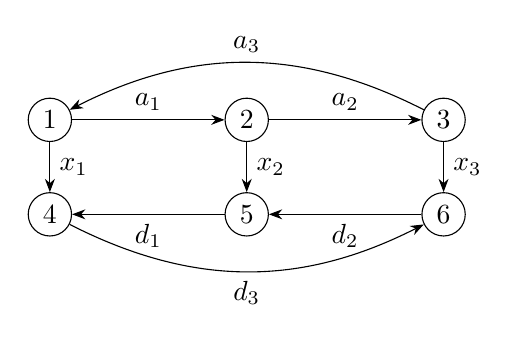
\begin{tikzpicture}[>=Stealth,
 vertex/.style={circle,draw,minimum size=5.5mm,inner sep=1pt}]
\node[vertex] (n1) at (0,1.2) {1};
\node[vertex] (n2) at (2.5,1.2) {2};
\node[vertex] (n3) at (5,1.2) {3};
\node[vertex] (n4) at (0,0) {4};
\node[vertex] (n5) at (2.5,0) {5};
\node[vertex] (n6) at (5,0) {6};
\draw[->] (n1) -- node[above] {\(a_1\)} (n2);
\draw[->] (n2) -- node[above] {\(a_2\)} (n3);
\draw[->] (n3) to[bend right=27] node[above] {\(a_3\)} (n1);
\draw[->] (n5) -- node[below] {\(d_1\)} (n4);
\draw[->] (n6) -- node[below] {\(d_2\)} (n5);
\draw[->] (n4) to[bend right=27] node[below] {\(d_3\)} (n6);
\draw[->] (n1) -- node[right] {\(x_1\)} (n4);
\draw[->] (n2) -- node[right] {\(x_2\)} (n5);
\draw[->] (n3) -- node[right] {\(x_3\)} (n6);
\end{tikzpicture}
\caption{The six-node construction. Nodes \(1,2,3\) are excited;
nodes \(4,5,6\) are measured. Each labeled edge has an independent
unknown coefficient.}
\label{fig:base}
\end{figure}

\begin{proposition}\label{prop:base}
The structure \eqref{eq:base} is generically locally identifiable in
\(\Omega\). For generic parameters, exactly two well-posed complex parameter
vectors give the same transfer matrix \(F\).
\end{proposition}

\begin{proof}
Assume first that \(x_1x_2x_3\ne0\), so that \(F\) is invertible.
Introduce coordinates \(u_i=a_i/x_i\), \(v_i=d_i/x_i\), and \(z_i=1/x_i\).
This change is invertible, with
\(a_i=u_i/z_i\), \(d_i=v_i/z_i\), and \(x_i=1/z_i\).
The inverse transfer matrix is
\begin{equation}\label{eq:Finverse}
\begin{split}
 F^{-1}&=(I_3-A)X^{-1}(I_3-D)\\
 &=\begin{pmatrix}
 z_1+u_3v_3/z_3&-v_1&-u_3\\
 -u_1&z_2+u_1v_1/z_1&-v_2\\
 -v_3&-u_2&z_3+u_2v_2/z_2
 \end{pmatrix}.
\end{split}
\end{equation}
Thus the off-diagonal entries determine \(u_i,v_i\).
Let \(e_i=(F^{-1})_{ii}\) be the diagonal entries. They satisfy
\begin{equation}\label{eq:diagonal}
 e_i=z_i+\frac{u_{i-1}v_{i-1}}{z_{i-1}}.
\end{equation}
With \(u_i,v_i\) fixed, the Jacobian of these three equations with
respect to \((z_1,z_2,z_3)\), denoted by \(J_z\), has determinant
\begin{equation}\label{eq:rankbase}
 \det J_z
 =1-\frac{u_1v_1u_2v_2u_3v_3}{z_1^2z_2^2z_3^2}
 =1-\alpha\delta.
\end{equation}
The six directly determined coordinates and \eqref{eq:rankbase} give
Jacobian rank nine when \(\alpha\delta\ne1\). Inverting an invertible
transfer matrix preserves rank. This proves generic local
identifiability.

To construct a second solution, define
\begin{equation}\label{eq:alternative}
\begin{split}
 k_i&=a_id_i\frac{x_{i+1}}{x_i},\qquad
 h_i=1+k_i+k_ik_{i+1},\\
 \eta_i&=\frac{k_ih_{i+1}}{h_i},\qquad
 (a_i',d_i',x_i')=\frac{1}{\eta_i}(a_i,d_i,x_i).
\end{split}
\end{equation}
Primes denote the alternative parameter values. The following identities
follow by expanding \(h_i\) and using \(k_1k_2k_3=\alpha\delta\):
\begin{equation}\label{eq:identities}
\begin{split}
 \eta_i-1&=\frac{\alpha\delta-1}{h_i},\\
 \eta_i+\frac{k_{i-1}}{\eta_{i-1}}&=1+k_{i-1},
 \qquad \eta_1\eta_2\eta_3=\alpha\delta.
\end{split}
\end{equation}
The transformation fixes \(u_i,v_i\) and gives \(z_i'=\eta_i z_i\).
Since \(u_{i-1}v_{i-1}/z_{i-1}=k_{i-1}z_i\), the second identity
in \eqref{eq:identities} preserves \eqref{eq:diagonal}, and hence \(F\).
The first identity makes the alternatives distinct when
\(\alpha\delta\ne1\). Denote the products of the primed cycle
coefficients by \(\alpha'=\prod_{i=1}^3a_i'\) and
\(\delta'=\prod_{i=1}^3d_i'\). The last identity gives
\begin{equation}\label{eq:products}
 \alpha'=\frac1\delta,\qquad \delta'=\frac1\alpha.
\end{equation}
Consequently the alternative is well posed whenever
\(\alpha\delta\ne0\) and \(\alpha,\delta\ne1\).

It remains to bound the number of solutions. Define \(b_i=u_iv_i\).
Equation~\eqref{eq:diagonal} gives successively
\[
 z_2=e_2-b_1/z_1,\quad
 z_3=e_3-b_2/z_2,\quad z_1=e_1-b_3/z_3.
\]
Substitution and multiplication by the denominators yield
\begin{equation}\label{eq:quadratic}
\begin{split}
0={}&(b_2-e_2e_3)z_1^2\\
 &+(b_1e_3-b_2e_1-b_3e_2+e_1e_2e_3)z_1\\
 &+b_1b_3-b_1e_1e_3.
\end{split}
\end{equation}
Generically its leading coefficient is nonzero, so there are at most
two values of \(z_1\). Each determines \(z_2,z_3\) and all original
parameters. A candidate with some \(x_i=0\) cannot yield an
invertible \(F\), by \eqref{eq:F}.
The rational formulas \eqref{eq:alternative} supply a distinct complex
second solution wherever the stated denominators are nonzero and
\(\alpha\delta\ne1\). These exclusions are zeros of nonzero polynomials.
For example, \(a_i=d_i=-1/2\) and \(x_i=1\) satisfy all of them.
This proves the assertion about exactly two solutions.
\end{proof}

The six-node construction alone does not give two alternatives in
\(\Omega_1\). Indeed, its block triangular form gives
\[
 \rho(G_b)=\max\{|\alpha|^{1/3},|\delta|^{1/3}\}.
\]
If both products have magnitude below one, \eqref{eq:products} makes
the alternative violate the same restriction. The next construction
changes the full network eigenvalues while retaining the ambiguity.

\section{Adding Excited and Measured Nodes \aicite}
\label{sec:augmentation}

Let \(w_b\in\mathbb C^6\) collect the original node amplitudes.
Add six nodes with amplitudes \(w_c\in\mathbb C^6\), all excited and measured.
Let \(K\in\mathbb C^{3\times6}\), \(L_c\in\mathbb C^{6\times3}\), and
\(J\in\mathbb C^{6\times6}\) specify the additional connections.
Define the augmented network and its selections by
\begin{equation}\label{eq:augmentation}
\begin{split}
 \mathcal G&=\begin{pmatrix}G_b&B_bK\\L_cC_b&J\end{pmatrix},\\
 \mathcal B&=\begin{pmatrix}B_b&0\\0&I_6\end{pmatrix},\qquad
 \mathcal C=\begin{pmatrix}C_b&0\\0&I_6\end{pmatrix}.
\end{split}
\end{equation}
This again has the form \eqref{eq:network}; its twelve node amplitudes
are the six original amplitudes \(w_b\) followed by \(w_c\).
The matrices \(K,L_c,J\) connect the added nodes to the original
excited and measured nodes and to each other.
Denote its transfer matrix by
\begin{equation}\label{eq:H}
 H=\mathcal C(I_{12}-\mathcal G)^{-1}\mathcal B.
\end{equation}

\begin{lemma}\label{lem:augmentation}
Suppose \(I_6-G_b\), \(X\), and \(I_{12}-\mathcal G\) are invertible.
Then \(H\) is invertible and
\begin{equation}\label{eq:Hinv}
 H^{-1}=\begin{pmatrix}F^{-1}&-K\\-L_c&I_6-J\end{pmatrix}.
\end{equation}
Consequently \(H\) determines each entry of \(K,L_c,J\), and, on this
domain, equality of augmented transfer matrices is equivalent to equality
of \(F,K,L_c,J\).
\end{lemma}

\begin{proof}
Let \(r_b\in\mathbb C^3\) and \(s\in\mathbb C^6\) be the input amplitudes
at the original and added nodes, respectively, and let \(y_b\in\mathbb C^3\)
be the original measured amplitudes. The node equations give
\[
 y_b=F(r_b+Kw_c),\qquad w_c=L_cy_b+Jw_c+s.
\]
Thus
\[
 \begin{pmatrix}r_b\\s\end{pmatrix}
 =\begin{pmatrix}F^{-1}&-K\\-L_c&I_6-J\end{pmatrix}
  \begin{pmatrix}y_b\\w_c\end{pmatrix}.
\]
By well-posedness, \((y_b,w_c)\) is obtained from \((r_b,s)\) through
the square matrix \(H\). The displayed matrix is therefore a left
inverse of \(H\), proving \eqref{eq:Hinv} and the remaining claims.
\end{proof}

This identity also preserves the rank information needed for local
identifiability. If \(q_c\) entries of \(K,L_c,J\) are independently
unknown and the remaining entries are fixed zeros, their derivatives
occupy positions in \eqref{eq:Hinv} disjoint from those of \(F^{-1}\).
The augmented Jacobian rank is therefore \(q_c+9\) wherever the base
Jacobian has rank nine. The choice below makes both compatible
augmented matrices satisfy the spectral-radius restriction.

\section{Ambiguity With Arbitrarily Small Spectral Radius \aicite}
\label{sec:main}

Use superscript \(T\) for transpose. Define the cyclic permutation
matrix \(U\), and then \(V\), by
\[
 U=\begin{pmatrix}0&0&1\\1&0&0\\0&1&0\end{pmatrix},
 \qquad V=U+U^T.
\]
These matrices satisfy
\(U^3=I_3\) and \(U^T=U^2\).
For real scalars \(t>0\) and \(x\ne0\), define
\begin{equation}\label{eq:M}
 M(t,x)=
 \begin{pmatrix}
 -tU&0&V&-U\\
 xI_3&-tU^T&0&0\\
 0&U^T&U^T&-V\\
 0&-V&I_3&U
 \end{pmatrix}.
\end{equation}
All blocks in this display have size \(3\times3\).
Use the nonzero positions in \(M(t,x)\) as the permitted edge set
for \(\mathcal G\). This pattern does not depend on the chosen
nonzero values of \(t,x\).
Assign a separate independent unknown coefficient to every permitted
position. There are nine in \(G_b\), nine in \(K\), nine in \(L_c\),
and fifteen in \(J\), giving \(m=42\).
Thus the repeated numerical values in \eqref{eq:M} specify particular
parameter choices in a class with forty-two independent complex coefficients.

The selections \(\mathcal B,\mathcal C\) in \eqref{eq:augmentation}
excite nodes 1--3 and 7--12 and measure nodes 4--12.
There are no diagonal edges.
Let \(\theta\in\mathbb C^{42}\) collect the independent coefficients
of this structure, and apply \eqref{eq:domain} to \(\mathcal G(\theta)\).

\begin{theorem}\label{thm:main}
For every \(0<\varepsilon\le1\), this twelve-node structure is
generically locally identifiable in \(\Omega_\varepsilon\).
There is a nonempty open set \(W_\varepsilon\subset\Omega_\varepsilon\)
such that every \(\theta\in W_\varepsilon\) has a distinct alternative
\(\widetilde\theta\in\Omega_\varepsilon\) with the same transfer matrix \(H\).
Both alternatives are locally identifiable. Consequently, the structure
is not generically globally identifiable in \(\Omega_\varepsilon\).
\end{theorem}

\begin{proof}
We first give equal transfer matrices, then make both spectral radii small,
and finally establish ambiguity on an open set of all forty-two
parameters.

\emph{Equal transfer matrices:}
The matrices in \eqref{eq:M} use the fixed numerical choices
\begin{equation}\label{eq:controller}
 K_0=\begin{pmatrix}V&-U\end{pmatrix},\quad
 L_0=\begin{pmatrix}U^T\\-V\end{pmatrix},\quad
 J_0=\begin{pmatrix}U^T&-V\\I_3&U\end{pmatrix}.
\end{equation}
For their base block, \(A=-tU\), \(D=-tU^T\), and \(X=xI_3\).
Write \(F(t,x)\) for the corresponding value of \eqref{eq:F}.
Since \(t>0\), the base block is well posed, and
\begin{equation}\label{eq:symmetric}
 F(t,x)^{-1}
 =x^{-1}(I_3+tU)(I_3+tU^T)
 =x^{-1}\big[(1+t^2)I_3+tV\big].
\end{equation}
Hence \(F(t,1)=F(t^{-1},t^{-2})\).
The two augmented matrices
\begin{equation}\label{eq:pair}
 \mathcal G_1(t)=M(t,1),\qquad
 \mathcal G_2(t)=M(t^{-1},t^{-2})
\end{equation}
use the same \(K_0,L_0,J_0\). By Lemma~\ref{lem:augmentation}, their
transfer matrices agree whenever both augmented networks are well posed.
They are distinct for \(t\ne1\).

\emph{Small spectral radii:}
At \(t=1\), both matrices in \eqref{eq:pair} equal \(M(1,1)\).
Let \(G_{b0}\) be its base block. Direct substitution gives
\[
 J_0=G_{b0}+B_bK_0-L_0C_b.
\]
Define the two matrices
\begin{equation}\label{eq:nilblocks}
\begin{split}
 E_+&=G_{b0}+B_bK_0
       =\begin{pmatrix}U^T&-U\\I_3&-U^T\end{pmatrix},\\
 E_-&=G_{b0}-L_0C_b
       =\begin{pmatrix}-U&-U^T\\I_3&U\end{pmatrix}.
\end{split}
\end{equation}
Changing coordinates from \((w_b,w_c)\) to \((w_b,w_b-w_c)\) makes
\(M(1,1)\) similar to the block upper triangular matrix
\begin{equation}\label{eq:triangular}
 \begin{pmatrix}E_+&-B_bK_0\\0&E_-\end{pmatrix}.
\end{equation}
The identities for \(U\) imply \(E_+^2=E_-^2=0\).
Squaring \eqref{eq:triangular} therefore gives a matrix whose only
possibly nonzero block is the upper right block; its square is zero.
Consequently
\begin{equation}\label{eq:nilpotent}
 M(1,1)^4=0.
\end{equation}

For a \(d\times d\) matrix \(Q\), let
\(\|Q\|_\infty=\max_{1\le i\le d}\sum_{j=1}^d|Q_{ij}|\), its maximum
absolute row sum.
The standard eigenvalue bound gives
\begin{equation}\label{eq:normbound}
 \rho(Q)^4=\rho(Q^4)\le\|Q^4\|_\infty.
\end{equation}
Both matrices in \eqref{eq:pair} converge to \(M(1,1)\) as \(t\to1\).
Their fourth-power norms consequently tend to zero.
For any prescribed \(0<\varepsilon\le1\), choose \(t\ne1\)
sufficiently close to one that both norms are below \(\varepsilon^4\).
Equation~\eqref{eq:normbound} then places both distinct matrices in
\(\Omega_\varepsilon\), so their transfer matrices are well defined and equal.

\emph{Local identifiability:}
The thirty-three independent added coefficients are determined directly
in \eqref{eq:Hinv}. The base Jacobian has rank nine by
\eqref{eq:rankbase}, since \(\alpha\delta=t^6\) at the first point of
\eqref{eq:pair} and \(\alpha\delta=t^{-6}\) at the second.
Both augmented Jacobians therefore have rank \(33+9=42\).
All their entries are rational functions of the forty-two parameters.
A minor, meaning the determinant of a square submatrix, that is
nonzero at one of these points has a numerator that is a
nonzero polynomial. Outside its zero set, the Jacobian of \(H\)
has full column rank. This establishes generic local identifiability
in \(\Omega_\varepsilon\).

\emph{An open set of ambiguous parameters:}
Define \(\mathcal T\) on the forty-two parameters by applying
\eqref{eq:alternative} to the nine base coefficients and leaving the
thirty-three added coefficients unchanged.
At the first point of \eqref{eq:pair}, one has \(k_i=t^2\),
\(h_i=1+t^2+t^4\), and \(\eta_i=t^2\); thus \(\mathcal T\) maps it to
the second point. All denominators are nonzero there.
The transformation is rational and continuous in a neighborhood, and
preserves \(H\) by Lemma~\ref{lem:augmentation}.

At these two points the fourth-power bounds are strict, the alternatives
are distinct, and both Jacobians have full column rank. These
properties persist in a sufficiently small open neighborhood
\(W_\varepsilon\) of the first point and its image under \(\mathcal T\).
Shrink the neighborhood further, if necessary, so that the base
inverses in the lemma exist and all permitted coefficients remain
nonzero. Then every
\(\theta\in W_\varepsilon\) and its alternative
\(\mathcal T(\theta)\) belong to \(\Omega_\varepsilon\), have equal
transfer matrices, and are distinct and locally identifiable.
The neighborhood is open in \(\mathbb C^{42}\), so it has positive
volume in the real and imaginary coordinates of \(\mathbb R^{84}\).
This disproves generic global identifiability.
\end{proof}

The conclusion also holds when all edge coefficients are restricted to
be real. The explicit pair in \eqref{eq:pair} is real, the transformation
\(\mathcal T\) preserves real coefficients, and its neighborhood contains
an open set of real parameters. The same rank argument proves generic
local identifiability on that real parameter domain.

\subsection{An explicit rational pair}

For \(\varepsilon=1\), choose \(t=99/100\) in \eqref{eq:pair}.
The common inverse transfer matrix, obtained from \eqref{eq:Hinv}, is
\begin{equation}\label{eq:commoninverse}
 H^{-1}=
 \begin{pmatrix}
 (1+t^2)I_3+tV&-V&U\\
 -U^T&I_3-U^T&V\\
 V&-I_3&I_3-U
 \end{pmatrix}.
\end{equation}
Exact multiplication of the rational matrices gives
\begin{equation}\label{eq:certificates}
\begin{split}
 \|\mathcal G_1(99/100)^4\|_\infty
     &=\frac{33910001}{100000000}<1,\\
 \|\mathcal G_2(99/100)^4\|_\infty
     &=\frac{16976126}{32019867}<1.
\end{split}
\end{equation}
These inequalities certify admissibility through \eqref{eq:normbound}.
Their spectral radii are approximately \(0.509563\) and \(0.404210\),
respectively. The exact equalities \eqref{eq:commoninverse} and
\eqref{eq:certificates} make the pair directly checkable with rational
arithmetic. Theorem~\ref{thm:main} establishes the open-set conclusion
independently of these numerical values.

\section{Transfer Functions and Conclusions \aicite}
\label{sec:conclusion}

\subsection{Algebraic identifiability over rational functions}

Let \(\lambda\) be a symbolic complex frequency variable and let
\(\mathbb K=\mathbb C(\lambda)\) be the field of ratios of polynomials
in \(\lambda\) with complex coefficients. We now replace the scalar
edge coefficients by elements of \(\mathbb K\), keeping the same
network structures and formulas for the transfer matrices. Each coordinate of
\(\theta\in\mathbb K^m\) is then a rational function of \(\lambda\).
Equality of transfer matrices means an identity of rational functions.

We use the algebraic framework of \cite[Sec.~V]{HMA26}.
For the algebraic calculation, the edge coordinates are independent
variables over \(\mathbb K\). Solutions are counted in an algebraic
closure \(\overline{\mathbb K}\), a field containing \(\mathbb K\)
in which every nonconstant polynomial has a root. An algebraic set is
a set defined by polynomial equations in these coordinates.
An algebraically generic property holds outside a proper algebraic
subset, meaning one smaller than the full parameter domain or the
image of the map \(\theta\mapsto\Phi(\theta)\), as appropriate.
The fiber at a transfer matrix is the set of admissible parameter
vectors producing it.
Generic local identifiability in the algebraic sense means that the
generic fiber has dimension zero, equivalently that it consists of
finitely many isolated points. Generic global identifiability requires
one point. Admissibility here excludes zeros of the determinants and
denominators required by the network equations.

In the notation of \cite{HMA26}, the matrices \(P,Q_r,R_y,S_{yr}\)
define the closed-loop transfer function \(R_yP^{-1}Q_r+S_{yr}\)
from external inputs to measured outputs.
Our augmented network is its specialization
\[
 P=I_{12}-\mathcal G,\qquad Q_r=\mathcal B,\qquad
 R_y=\mathcal C,\qquad S_{yr}=0.
\]

\begin{proposition}\label{prop:field}
Over \(\mathbb K\), the six-node structure \eqref{eq:base} and the
twelve-node structure of Theorem~\ref{thm:main} each have exactly
two points in the generic algebraic fiber. Both are therefore
generically locally identifiable in the algebraic sense and fail
generic global identifiability. If one generic parameter vector has
coordinates in \(\mathbb K\), its distinct alternative also has
coordinates in \(\mathbb K\).
\end{proposition}

\begin{proof}
All identities in Proposition~\ref{prop:base} use only field
operations and remain valid over \(\overline{\mathbb K}\).
The quadratic \eqref{eq:quadratic} permits at most two base solutions.
Formula~\eqref{eq:alternative} provides a distinct second solution
outside the stated algebraic exclusions. Because this formula is
rational, it maps \(\mathbb K\)-valued parameters to
\(\mathbb K\)-valued parameters.

For a generic transfer matrix \(H\), both \(H\) and the upper left
\(3\times3\) block of \(H^{-1}\) are invertible.
Any well-posed candidate producing this \(H\) must have invertible
\(X\). Otherwise choose a nonzero vector
\(\xi\in\overline{\mathbb K}^3\) with \(X\xi=0\).
The node amplitudes \((\xi,0,0)\), partitioned into groups of sizes
three, three, and six, give zero output for input
\(((I_3-A)\xi,0)\). Well-posedness makes this input nonzero,
contradicting invertibility of \(H\).
Eliminating the first three node amplitudes now gives
\[
 H^{-1}=
 \begin{pmatrix}
 (I_3-A)X^{-1}(I_3-D)&-K\\
 -L_c&I_6-J
 \end{pmatrix}.
\]
Invertibility of its upper left block makes \(I_3-A\) and
\(I_3-D\) invertible. Hence every candidate satisfies the lemma's
assumptions. The added coefficients are determined, and the remaining
fiber is exactly the two base solutions. For either base solution,
the displayed invertible matrix determines the measured node amplitudes
from the inputs, and \(X^{-1}(I_3-D)\) determines the first three
node amplitudes. Thus both augmented solutions are well posed.
The transformation \(\mathcal T\) leaves the added coefficients
unchanged, so it also preserves \(\mathbb K\)-valued parameters.
\end{proof}

\subsection{Properness and spectral-radius restrictions}

A rational transfer function is \emph{proper} if its numerator
degree does not exceed its denominator degree, and
\emph{strictly proper} if the inequality is strict.
Each real coefficient in \eqref{eq:pair} defines a constant proper
rational transfer function.
The matrix \((I_{12}-\mathcal G)^{-1}\), which maps additive inputs
at all nodes to the node signals, is also constant. It maps bounded
inputs to bounded signals, so the network is stable in this
input-output sense. Both networks have identical transfer matrices
and satisfy the spectral-radius restriction at every frequency.

Algebraically generic uniqueness also fails after imposing properness,
stability, and the spectral-radius bound.
Indeed, \(W_\varepsilon\cap\mathbb R^{42}\) from
Theorem~\ref{thm:main} contains a nonempty real open set of ambiguous
constant networks. This set is Zariski dense over
\(\overline{\mathbb K}\), meaning that no nonzero polynomial in the
forty-two edge coordinates vanishes on all of it.
To see this, take a real open box contained in the set. Fix all but
one coordinate in their respective intervals. A polynomial vanishing
throughout the box has infinitely many roots in the remaining
coordinate, so each of its coefficients is zero. Repeating this
argument for the other coordinates proves that the polynomial is zero.
Thus no proper algebraic exceptional set can contain all these
admissible ambiguous networks.
Their transfer matrices are also Zariski dense in the image of
the map \(\theta\mapsto H(\theta)\).
Indeed, suppose a polynomial vanishes on all these transfer matrices but
not on the full image. Substituting \(H(\theta)\) and clearing
denominators gives a nonzero polynomial that vanishes on the real
open set, a contradiction.

This conclusion uses the edge transfer functions themselves as
coordinates over \(\mathbb K\). A separate analysis is required
when genericity refers to the numerical coefficients of a prescribed
positive-order transfer-function family, or when the admissible
networks must be strictly proper.

The construction separates local recovery from global uniqueness even
under an arbitrarily small positive spectral-radius bound. Its mechanism
is explicit: the six-node equations admit two isolated solutions, and
the added excited and measured nodes preserve those solutions while
moving all eigenvalues of both complete networks near zero. Thus a derivative rank
test for local identifiability cannot establish generic global
identifiability for this class of partially excited and measured
networks.

\clearpage
\balance
\section*{Acknowledgment}
OpenAI Codex \cite{codex} assisted in developing the construction and
proofs, writing symbolic verification code, and drafting and editing
the abstract and Sections~\ref{sec:intro}--\ref{sec:conclusion}.
The citations in the section headings identify text drafted with this
assistance.

\begin{thebibliography}{9}
\bibitem{codex}
OpenAI, \lq\lq Codex,'' software.
[Online]. Available: \url{https://openai.com/codex/}.
Accessed: Oct.~8, 2026.

\bibitem{LH20}
A.~Legat and J.~M.~Hendrickx, \lq\lq Local network identifiability with
partial excitation and measurement,'' in \emph{Proc. 59th IEEE Conf.
Decision Control}, 2020, pp.~4342--4347,
doi:~\href{https://doi.org/10.1109/CDC42340.2020.9303890}
{10.1109/CDC42340.2020.9303890}.

\bibitem{LH24}
A.~Legat and J.~M.~Hendrickx, \lq\lq Identifiability in networked systems:
Algebraic and combinatorial conditions,'' manuscript, 2024.
[Online]. Available:
\url{https://perso.uclouvain.be/antoine.legat/_static/TAC24.pdf}.

\bibitem{LH23}
A.~Legat and J.~M.~Hendrickx, \lq\lq Combinatorial characterization for
global identifiability of separable networks with partial excitation
and measurement,'' in \emph{Proc. 62nd IEEE Conf. Decision Control},
2023, pp.~2471--2476,
doi:~\href{https://doi.org/10.1109/CDC49753.2023.10383708}
{10.1109/CDC49753.2023.10383708}.

\bibitem{L25}
A.~Legat, \lq\lq Generic local identifiability in dynamical networks: From
algebraic characterization to algorithms for signal selection,''
Ph.D. dissertation, UCLouvain, Louvain-la-Neuve, Belgium, 2025.
[Online]. Available: \url{https://hdl.handle.net/2078.5/256546}.

\bibitem{HMA26}
A.~Hansson, J.~V.~Galv{\~a}o da Mata, and M.~S.~Andersen,
\lq\lq Informativity and identifiability for identification of
networks of dynamical systems,'' arXiv:2602.20107, 2026.
[Online]. Available: \url{https://arxiv.org/abs/2602.20107v3}.
\end{thebibliography}
\end{document}
